\documentclass{beamer}
\mode<presentation> {
\usetheme{Boadilla}
\setbeamercovered{invisible}
\setbeamertemplate{navigation symbols}{} 
}

%\newcommand{\abs}[1]{\ensuremath{\left|#1\right|}}
%\newcommand{\bracket}[2]{\ensuremath{\left\langle#1 \vphantom{#2}\middle|  #2 \vphantom{#1}\right\rangle}}

\usepackage{amsmath, amsfonts, amssymb}
\usepackage{graphicx}
\title[HCA]{Hierarchical Controller Architecture for SDN}
\author[]{\textbf{Gourav Khaneja\\Sweta Yamini Seethamraju} \\ \small{Supervisor:} Prof. Philip Brighten Godfrey}
\date{\today}

\begin{document}
\frame{
\titlepage
}

\frame{
\frametitle{Outline}
\tableofcontents
}

\section{Introduction}

\frame{
\frametitle{Problem}
\begin{itemize}
	\item Single controller architecture is not scalable
	\item Distributed controller architectures provide global view to control application
\pause
	\item Problems are
	\begin{itemize}
		\item Communication overhead
		\item Network state inconsistencies
		\item Management barriers across networks 
		\item Scalability of complete global view of the network
	\end{itemize}
\pause
	\item Trade-offs
	\begin{itemize}
		\item Consistency vs. Responsiveness
		\item Application design complexity (architecture aware vs. agnostic)
	\end{itemize}
\pause
	\item Aim
	\begin{itemize}
		\item Make control application agnostic to underlying distributed architecture
		\item Aggregate network to simplify network view
		\item Handle inconsistency in "SDN datapath"
	\end{itemize}
\end{itemize}
}

\frame{
\frametitle{Previous Work}
\begin{itemize}
	\item Hyperflow
\pause
	\begin{itemize}
		\item Flat distributed controller architecture
		\item Appliations are agnostic to underlying state distribution
		\item Provides a logically centralized global view of the network
		\item Results in performance degradation and transient inconsistencies
	\end{itemize}
\pause
	\item Onix
\pause
	\begin{itemize}
		\item Provides flexible framework to handle controller topology
		\item Provides generic distributed state management API
		\item Provides a framework but not an approach
		\item Design decisions left to control application
	\end{itemize}
\pause
	\item Kandoo
\pause
	\begin{itemize}
		\item Two-level controller architecture
		\item Events are propagated only on subscription
		\item Applications need to be aware of hierarchy
		\item View of root controller varies with control application
	\end{itemize}
\end{itemize}
}

\section{Approach}

\frame{
\frametitle{What }
\begin{itemize}
	\item
\end{itemize}
}


\frame{
\frametitle{Our Approach}
\begin{itemize}
	\item
\end{itemize}
}



\section{Progress}

\frame{
\frametitle{Progress}
\begin{itemize}
	\item
\end{itemize}
}

\frame{
\frametitle{Results}
\begin{itemize}
\item Preliminary link utilization plots
\end{itemize}
\begin{figure}
 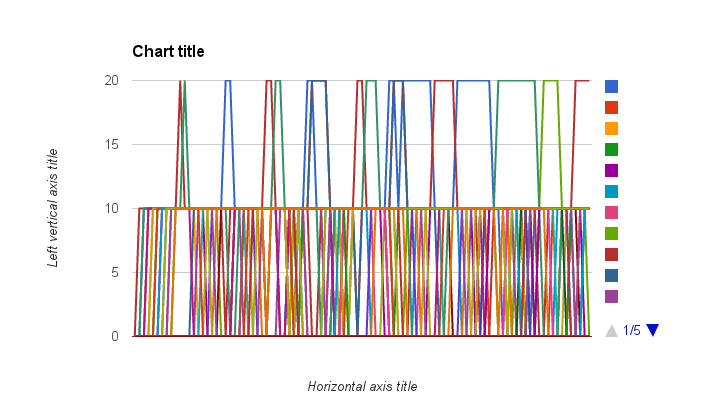
\includegraphics[scale=0.2]{../chart_1}
\caption{Link utilization}
\end{figure}
}

\frame{
\frametitle{Future Work}
\begin{itemize}
	\item 
	\item Implement using OpenFlow
\end{itemize}
}

\frame{
\centerline{Thank you!}
}

\end{document} 
